\documentclass[xcolor=table]{beamer}
\mode<presentation>

\usepackage{ulem}
\usepackage[T1]{fontenc}
\usepackage[scaled=0.85]{beramono}
\usepackage{framed}
\usepackage{listings}


\usepackage{tikz}
\usetikzlibrary{shapes}
\usetikzlibrary{positioning,arrows,shadows,decorations.pathreplacing}

\setbeamertemplate{navigation symbols}{}
\usetheme{Boadilla}
\usecolortheme{beaver}
\usefonttheme{serif}

\linespread{1.5}

\title{Quantatative and Qualatative Qualities of Contemporary Capability Constructions}
\date{Feb 26, 2016}
\author{Kritika Iyer, Sajin Sasy, Justin Tracey}

\begin{document}

\begin{frame}
  \titlepage
  \centering
  CS 854
\end{frame}

\begin{frame}
  \frametitle{Access Control}
  \begin{itemize}
  \item Systems, including Operating Systems, control resources.
  \item How do they designate who gets access to what resource?
  \item Answer: Access Control Tables
  \end{itemize}
\end{frame}

\begin{frame}
  \frametitle{Example Access Control Table}
  \begin{center}
    \begin{tabular}{|l||c|c|c|}
      \hline
      &File 1&File 2&File 3\\
      \hline
      \hline
      Alice&rw&rx&rwx\\
      \hline
      Bob&&rx&\\
      \hline
      Carol&r&rx&\\
      \hline
    \end{tabular}\\
    \vspace{10pt}
    \invisible{Line here for consistent spacing}
  \end{center}
\end{frame}

\begin{frame}
  \frametitle{Access Control Representation}
  How is this table actually represented?
  \begin{itemize}
  \item Representing the entire table is wasteful... \pause
  \item Access Control Lists
  \item Capabilities
  \end{itemize}
\end{frame}

\begin{frame}
  \frametitle{Access Control Lists}
  \begin{center}
    \begin{tabular}{|l||c|c|c|}
      \hline
      &\cellcolor{green}File 1&File 2&File 3\\
      \hline
      \hline
      Alice&\cellcolor{green}rw&rx&rwx\\
      \hline
      Bob&\cellcolor{green}&rx&\\
      \hline
      Carol&\cellcolor{green}r&rx&\\
      \hline
    \end{tabular}\\
    \vspace{10pt}
    ``I am File 1. Alice has rw permissions, Carol has r permissions.''
  \end{center}
\end{frame}

\begin{frame}
  \frametitle{Capabilities}
  \begin{center}
    \begin{tabular}{|l||c|c|c|}
      \hline
      &File 1&File 2&File 3\\
      \hline
      \hline
      Alice&rw&rx&rwx\\
      \hline
      Bob&&rx&\\
      \hline
      \cellcolor{green}Carol&\cellcolor{green}r&\cellcolor{green}rx&\cellcolor{green}\\
      \hline
    \end{tabular}\\
    \vspace{10pt}
    ``I am Carol, with r permissions for File 1, and rx permissions for File 2.''
  \end{center}
\end{frame}

\begin{frame}
  \frametitle{The 4 Types of Capability Systems}
  
\begin{enumerate}
    \item{Tagged with bits}
    \item{Tagged with type system}
    \item{Segregated}
    \item{Password/ Sparse}
\end{enumerate}
 \end{frame}

\begin{frame}
    \frametitle{Present Implementations: Kernel Space}
     \begin{itemize}
         \item Operating Systems :
         \begin{itemize}
             \item KeyKOS
             \item L4 Family : sel4 , Fiasco.OC
             \item Barrelfish
             \item Linux
         \end{itemize}
     \end{itemize}
\end{frame}

\begin{frame}{Present Implementations: User space}
\begin{itemize}
    \item Programming languages to implement capability security:
    \begin{itemize}
        \item Joule
        \item E
        \item Joe-E
        \item Caja project
    \end{itemize}

    \item User space capability system:
    \begin{itemize}
        \item capBAC
    \end{itemize}
\end{itemize}

\end{frame}

\begin{frame}
  \frametitle{Open Problems}
    \begin{itemize}
        \item Existing systems do not always scale to new paradigms (IoT)
        \item Performance measurements are scarce 
    \end{itemize}
 
\end{frame}

\begin{frame}
  \frametitle{Our Goals}
   \begin{itemize}
      \item Conduct survey of existing systems and implementations of capability-based security
      \item Record performance metrics for comparing different systems and implementations
      \item Identify which systems work well with new use-cases
      \item Identify ways to optimize results for existing use-cases
      
      
  \end{itemize}
\end{frame}

\begin{frame}{OrangeFS}
    \begin{itemize}
    \vfill
    \item Certificate based file system
    \vfill
    \item Model of capability with tagged bits
    \vfill
    \item Data stored in clear
    \vfill
    \end{itemize}
   % \begin{figure}
	%	  \includegraphics[scale=0.25]{orange.png}
	%	  \caption{OrangeFS}
    %\end{figure}
    \begin{textblock*}{4cm}(8cm,3cm)
        \includegraphics[width=3cm]{img/orange.png}
    \end{textblock*}
\end{frame}

\begin{frame}{TahoeLAFS}
    \begin{itemize}
    \vfill
    \item Password based capability mode
    \vfill
    \item Mutable and Immutable files
    \vfill
    \item Directory Logic
    \vfill
    \end{itemize}
\end{frame}

\begin{frame}{TahoeLAFS (Immutable files)}
    \vfill
    \begin{itemize}
    \item Immutable Files
    \end{itemize}
    \vfill
    \begin{figure}
		  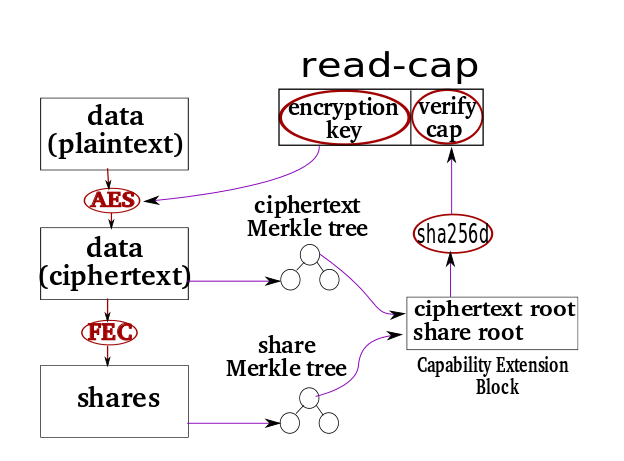
\includegraphics[scale=0.5]{img/immutable.png}
		  \caption{Revoke-Retype-Delete interactions}
    \end{figure}
    \vfill
    % insert 1 diagram
\end{frame}

\begin{frame}{TahoeLAFS (Mutable files)}
    \vfill
    \begin{itemize}
    \item Mutable Files
    \end{itemize}
    \vfill
    \begin{figure}
		  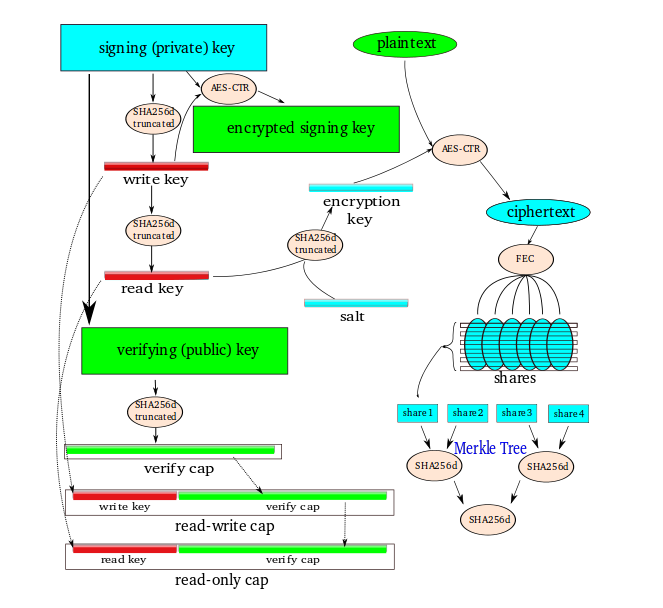
\includegraphics[scale=0.5]{img/mutable.png}
		  \caption{Revoke-Retype-Delete interactions}
    \end{figure}
    \vfill
\end{frame}

\begin{frame}{CapBAC}
    \begin{itemize}
    \vfill
    \item Designed for the Internet of Things
    \vfill
    \item JSON-file Tokens
    \vfill
    \end{itemize}
    \begin{textblock*}{2.5cm}(8cm,1.5cm)
        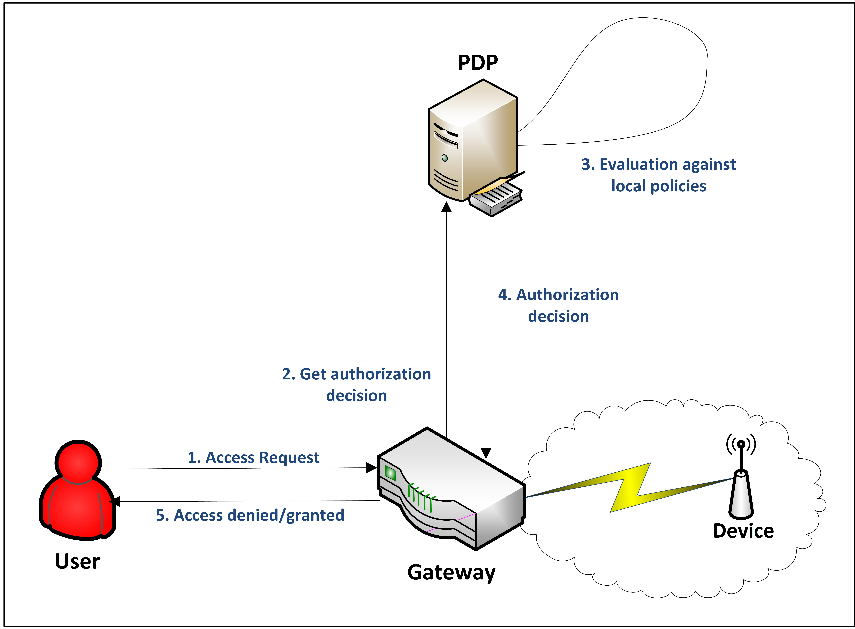
\includegraphics[width=2cm]{img/centralized.png}
    \end{textblock*}
    \begin{textblock*}{2.5cm}(8cm,4cm)
        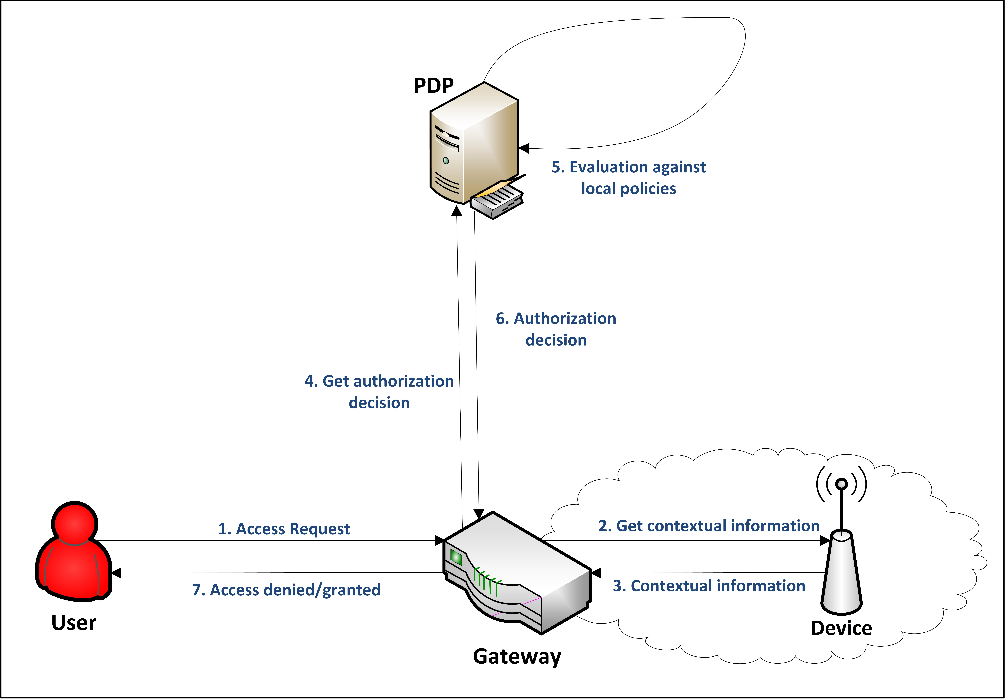
\includegraphics[width=2cm]{img/CAcentralized.png}
    \end{textblock*}
    \begin{textblock*}{2.5cm}(8cm,6.5cm)
        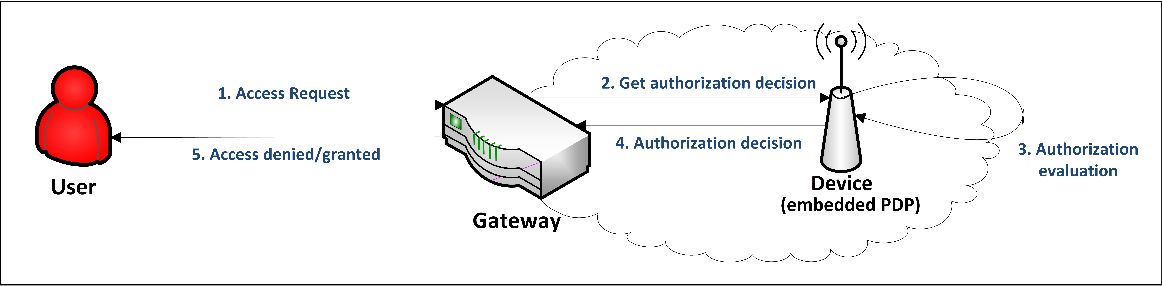
\includegraphics[width=2cm]{img/distributed.png}
    \end{textblock*}
    % insert 3 diagrams (centralized, CAcentralized, distributed)
\end{frame}

\begin{frame}{CapBAC}
    \vfill
    \begin{itemize}
    \item Implementation Model 
    \end{itemize}
        \vfill
    \begin{figure}
		  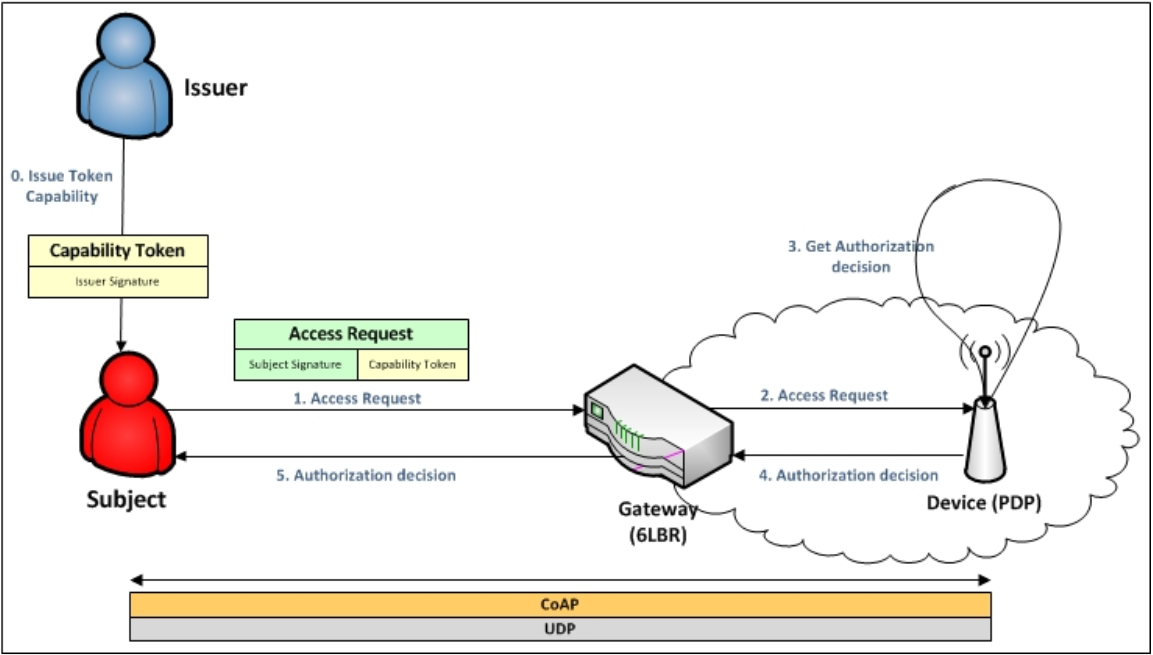
\includegraphics[scale=0.5]{img/capBac.png}
		  \caption{Revoke-Retype-Delete interactions}
    \end{figure}
    \vfill
    % insert 1 diagram capBAC
\end{frame}

\end{document}
